\chapter{Resultados y discusión}

En este capítulo se muestran los resultados obtenidos de aplicar las rutinas desarrolladas con anterioridad.



\section{Test de respuesta conocida}
Este test se realiza para comprobar que la compilación e integración de los algoritmos funciona matemáticamente igual que las implementaciones de referencia presentadas al \acrshort{nist}. Para ello, el procedimiento estándar en un \textit{Known Answer Tests} consiste en generar un fichero de respuesta (\texttt{.rsp}) a partir de una semilla inicial fija con la cual mediante el generador \texttt{rng.h} pseudoaleatorio se derivan todas las claves y textos cifrados. Si la implementación es correcta el fichero ha de ser igual al proporcionado por los autores.
\subsection{Kyber}
La ejecución de los tests para Kyber se completó sin incidencias. Se procesaron los 100 vectores de prueba definidos por el NIST. Al utilizar la misma semilla de entrada, la implementación generó claves y criptogramas idénticos a la referencia.



%En el Listing \ref{lst:kyber_kat} se muestra el primer vector de prueba generado por nuestra implementación, donde se verificó la coincidencia exacta de la clave pública (\texttt{pk}), la clave secreta (\texttt{sk}) y el secreto compartido (\texttt{ss}) con los valores esperados.
%\begin{lstlisting}[caption={Extracto del fichero .rsp generado para Kyber (Vector 0)}, label={lst:kyber_kat}, basicstyle=\ttfamily\scriptsize]
%	# kyber512
%	count = 0
%	seed = 632616E53E5C162547070F037A3C4D2644D25C6552272846174A698762514332
%	pk = 753F88E022567D07...[truncado]...A3273187FDD077
%	sk = 826F8082692F0197...[truncado]...A3273187FDD077
%	ct = 7219927A685D26C3...[truncado]...E5D79E182D2D70
%	ss = A3D3F1E38367A58E29E250A84D5852267667C08CC3B44B36398F81716A8C576D
%\end{lstlisting}
\subsection{Saber}
\subsection{HQC}
\section{CPU cicles}
\subsection{Comparacion por plataforma}
\begin{figure}[H]
	\centering
	\includegraphics[width=1\linewidth]{figuras/cycles_platform}
	\caption{}
	\label{fig:cyclesplatform}
\end{figure}

\subsection{Comparacion por algoritmo}
\begin{figure}[H]
	\centering
	\includegraphics[width=1\linewidth]{figuras/cycles_device}
	\caption{}
	\label{fig:cyclesdevice}
\end{figure}

\section{Throughput}
\subsection{Comparacion por plataforma}
\begin{figure}[H]
	\centering
	\includegraphics[width=1\linewidth]{figuras/throughput_platform}
	\caption{}
	\label{fig:throughputplatform}
\end{figure}

\subsection{Comparacion por algoritmo}
\begin{figure}[H]
	\centering
	\includegraphics[width=1\linewidth]{figuras/throughput_device}
	\caption{}
	\label{fig:throughputdevice}
\end{figure}

\section{Uso de pila}
\subsection{Comparacion por plataforma}
\begin{figure}[H]
	\centering
	\includegraphics[width=1\linewidth]{figuras/stack_platform}
	\caption{}
	\label{fig:stackplatform}
\end{figure}

\subsection{Comparacion por algoritmo}
\begin{figure}[H]
	\centering
	\includegraphics[width=1\linewidth]{figuras/stack_device}
	\caption{}
	\label{fig:stackdevice}
\end{figure}
\section{Coste de comunicación y tiempo teórico de ejecución de los protocolos}
\section{Test de aleatoriedad}
\subsection{Plataforma Windows}
\begin{figure}[H]
	\centering
	\includegraphics[width=0.7\linewidth]{figuras/1_histogramWIN}
	\caption{}
	\label{fig:1histogramwin}
\end{figure}
\begin{figure}[H]
	\centering
	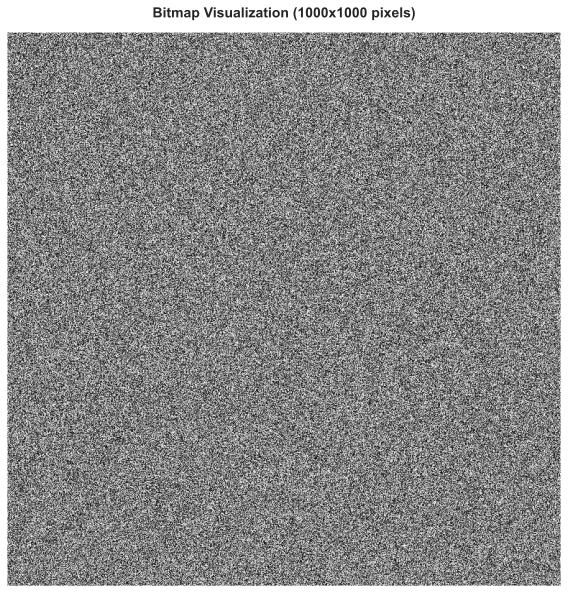
\includegraphics[width=0.7\linewidth]{figuras/2_bitmapWIN}
	\caption{}
	\label{fig:2bitmapwin}
\end{figure}
\begin{figure}[H]
	\centering
	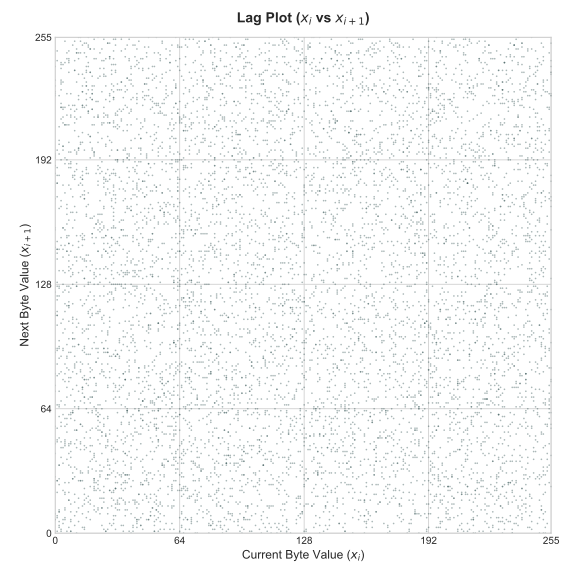
\includegraphics[width=0.7\linewidth]{figuras/3_lagplotWIN}
	\caption{}
	\label{fig:3lagplotwin}
\end{figure}

\subsection{PSOC}
\begin{figure}[H]
	\centering
	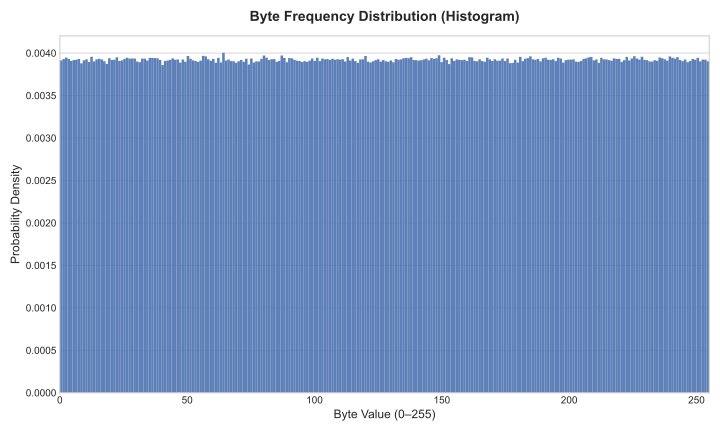
\includegraphics[width=0.7\linewidth]{figuras/1_histogramPSOC}
	\caption{}
	\label{fig:1histogrampsoc}
\end{figure}
\begin{figure}[H]
	\centering
	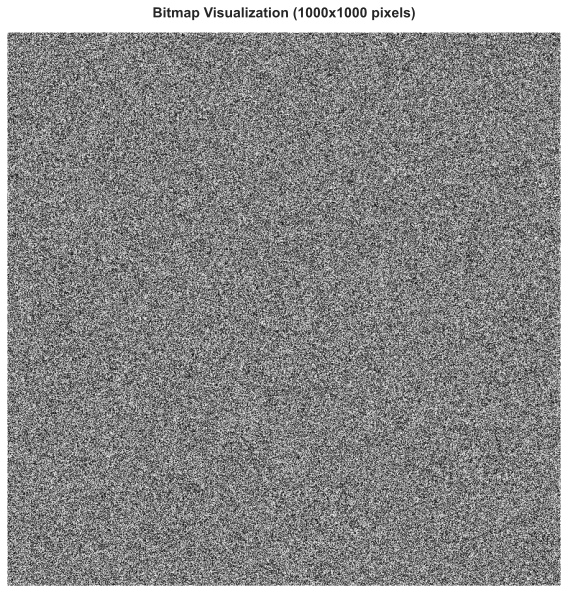
\includegraphics[width=0.7\linewidth]{figuras/2_bitmapPSOC}
	\caption{}
	\label{fig:2bitmappsoc}
\end{figure}
\begin{figure}[H]
	\centering
	\includegraphics[width=0.7\linewidth]{figuras/3_lagplotPSOC}
	\caption{}
	\label{fig:3lagplotpsoc}
\end{figure}
